This chapter presents an evaluation of \bpfbox{} and \bpfcontain{} in terms of their
performance and security. \Cref{s:eval-performance} presents the methodology and results
of a performance evaluation involving micro- and macro-benchmarking of \bpfbox{} and
\bpfcontain{}. Results are compared with AppArmor~\cite{cowan2000_apparmor}, a popular
\gls{lsm} framework for \gls{mac} security policy. Finally, \Cref{s:eval-security}
presents a security analysis of \bpfbox{} and \bpfcontain{} under the threat model
outlined in \Cref{s:cp-threat-model} of \Cref{c:confinement-problem}.

\section{Performance Evaluation}%
\label{s:eval-performance}

This section presents a performance evaluation of \bpfbox{} and \bpfcontain{}, measuring
their performance overhead using a variety of micro- and macro-benchmarking tests. In
particular, we leverage the Phoronix Test Suite~\cite{phoronix} to measure overhead across
a variety of computational tasks, workloads, and kernel interfaces. Each of these
benchmarks exercises a different subset of \bpfbox{} and \bpfcontain{}'s enforcement
engine, providing an approximation of their impact on the overall system. We also measure
the performance of the base system as a control, and the performance overhead of AppArmor
as a basis for direct comparison. The subsections that follow provide an overview of the
testing methodology and present the benchmark results.

\subsection{Methodology}%
\label{ss:eval-methodology}

As a test environment, we utilize a bare-metal system running Arch Linux with a stock
5.12.14-arch-1-1 kernel. The choice of a bare-metal system (rather than a virtual machine,
for instance) reduces the risk of introducing additional sources of variance into the
benchmarks. \Cref{tab:system-config} provides a detailed account of the test system
configuration.

\begin{table}[htpb]
  \centering
  \caption[System configuration for benchmarking tests]{System configuration for benchmarking tests.}%
  \label{tab:system-config}
  \begin{tabular}{ll}
  \toprule
  Item & Description / Configuration \\
  \midrule
  CPU & Intel i7-10875H; 8 cores, 16 threads at 2.3GHz; 16MB cache\\
  GPU & Nvidia RTX 2060 with 6GB GDDR6 VRAM \\
  RAM & 2$\times$16GB DDR4 at 3.2GHz \\
  Disk & 1TiB Samsung NVME M.2 SSD \\
  \midrule
  \gls{os} & Arch Linux (Rolling) \\
  Kernel & Linux v5.12.14-arch-1-1 \\
  Libc & glibc v2.33-5 \\
  Phoronix & v10.4.0-1 \\
  \bottomrule
  \end{tabular}
\end{table}

To simulate the Docker container use case, we run all tests in a privileged Docker
container, using Docker volumes to mount the host filesystem in the benchmarking
directory. To improve benchmarking accuracy, we also perform the following setup before
each test. (1) We disable SMT hyperthreading by turning off each logical CPU core pair,
leaving only the physical cores active; (2) We disable turbo boost, capping the CPU at its
stock speed of 2.3GHz; (3) We set the CPU frequency scaling governor to
\enquote{performance} to limit the impact of thermal throttling and power saving features;
and (4) We globally disable \gls{aslr} by setting the appropriate kernel parameter. These
settings, consistent with best practices, improve benchmark accuracy by making the
environment more consistent and eliminating as many external factors as possible.

To measure the performance overhead of \bpfbox{} and \bpfcontain{} (compared with the base
system and with AppArmor) we leverage the Phoronix Test Suite~\cite{phoronix}, a popular
cross-platform benchmarking framework that has seen wide use for measuring system
performance. The Phoronix framework comprises a number of open source test suites, each
targeting a different aspect of system behaviour. For the purposes of this thesis, we
select three separate test suites, measuring a variety of \gls{os}-level functionality and
exercising multiple \gls{lsm} hooks. In particular, we select the OSBench suite, the
Kernel Compilation suite, and the Apache suite. \Cref{tab:suites} describes each test
suite and what it measures.

\begin{table}[htpb]
  \centering
  \caption[List of benchmarking suites and what they measure]{
    A list of the benchmarking suites used to test performance overhead and what each
    measures.
  }%
  \label{tab:suites}
  \begin{tabular}{llp{3in}}
  \toprule
  Test Suite & Test & Measures \\
  \midrule
  OSBench                    & Create Files       & Time to create and delete files \\
                             & Create Threads     & Time to create new threads \\
                             & Launch Programs    & Time to fork + execve \\
                             & Create Processes   & Time to create new processes \\
                             & Memory Allocations & Memory allocation throughput \\
  Kernel Compilation         & ---                & Time to compile Linux Kernel \\
  Apache Web Server          & ---                & Apache HTTP request throughput \\
  % \gls{ipc}                  & Unix Socket        & Unix socket throughput \\
  %                            & TCP Socket         & TCP socket throughput  \\
  %                            & Named Pipe         & Named pipe throughput  \\
  %                            & Unnamed Pipe       & Unnamed pipe throughput \\
  \bottomrule
  \end{tabular}
\end{table}

We consider ten system configurations in total (\Cref{fig:configuration}). The
\textbf{Base} configuration is the base system without any \glspl{lsm} or other
confinement primitives active or loaded in the kernel. The \textbf{\bpfbox},
\textbf{\bpfcontain}, and \textbf{AppArmor} configurations measure the performance
overhead of \bpfbox{}, \bpfcontain{}, and AppArmor, respectively. We then divide each of
these three configurations into three distinct test cases each. The \textbf{Passive} case
measures global system overhead without any active enforcement. The \textbf{Allow} case
measures active enforcement, allowing all security-sensitive operations. Finally, the
\textbf{Complain} case measures the worst-case overhead for each system, exercising the
full code path of each \gls{lsm} hook and logging every attempted access.

\begin{figure}[htp]
  \centering
  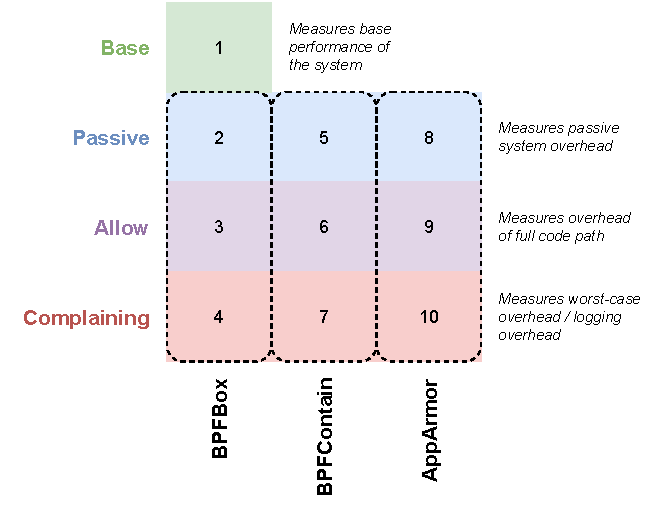
\includegraphics[width=0.6\linewidth]{figs/eval/configuration.pdf}
  \caption[Benchmarking system configurations]{
    The various system configurations used in the benchmarking tests.
  }%
  \label{fig:configuration}
\end{figure}

To ensure statistically valid results, we run each test at least eleven times, until
a standard deviation of at most $2\%$ is achieved. We also discard the first run of each
test to control for initial I/O transients. In total, the result is at least ten trials
for each test suite and system configuration. For reproducibility, we make the
benchmarking repository publicly available\footnote{Benchmarking tests are available:
\url{https://github.com/willfindlay/bpfcontain-benchmarks}}, including all results and
related scripts.

% \begin{inprogress}
%   \begin{itemize}
%     \item Test environment
%     \begin{itemize}
%       \item Describe system specs
%       \item To improve benchmark accuracy, we disable ...
%       \item We run tests in a privileged Docker container
%       \item Arch Linux Kernel 5.12.15-arch-1
%     \end{itemize}

%     \item Phoronix Test Suite tests
%     \begin{itemize}
%       \item \todo{Describe each test in detail and explain what LSM hooks it exercises}
%     \end{itemize}

%     \item \todo{Other tests if we have time}

%     \item Explain each test case (base, \{bpfbox, bpfcontain, apparmor\}, \{passive, allow, complaining\})
%     \item Run reach test for at least 11 trials, until we achieve an acceptable standard deviation ($<2\%$)
%     \item Discard first run of each trial, to control for initial I/O transients and caching
%     \item Reproducibility, give \bpfbox{} and \bpfcontain{} version, with tags on GitHub
%     \item Link to the benchmarking repo

%   \end{itemize}
% \end{inprogress}

\subsection{Results}%
\label{ss:eval-results}

This section presents the results of the OSBench micro-benchmarks
(\Cref{fig:osbench-results} and \Crefrange{tab:phoronix-files}{tab:phoronix-memory}) and
the kernel compilation (\Cref{fig:phoronix-kernel} and \Cref{tab:phoronix-kernel}) and
Apache web server (\Cref{fig:phoronix-apache} and \Cref{tab:phoronix-apache})
macro-benchmarks. We find that \bpfbox{} and \bpfcontain{} perform competitively with
AppArmor in most cases, with \bpfcontain{} experiencing minor performance degradations in
some cases, which can be attributed to \bpfcontain{}'s status as a research prototype.  In
light of these results, we discuss how future optimizations to \bpfcontain{} and the
\gls{krsi} framework can greatly improve its performance overhead in practice.

\begin{figure}[htp]
  \centering
  \subfloat{
    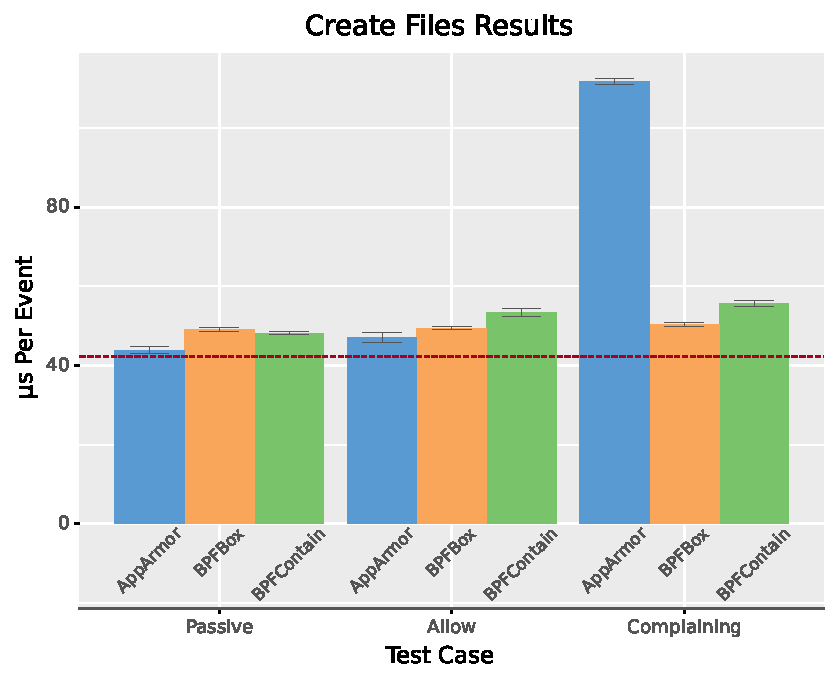
\includegraphics[width=0.45\linewidth]{results/graphs/Create-Files.pdf}%
  }\qquad
  \subfloat{
    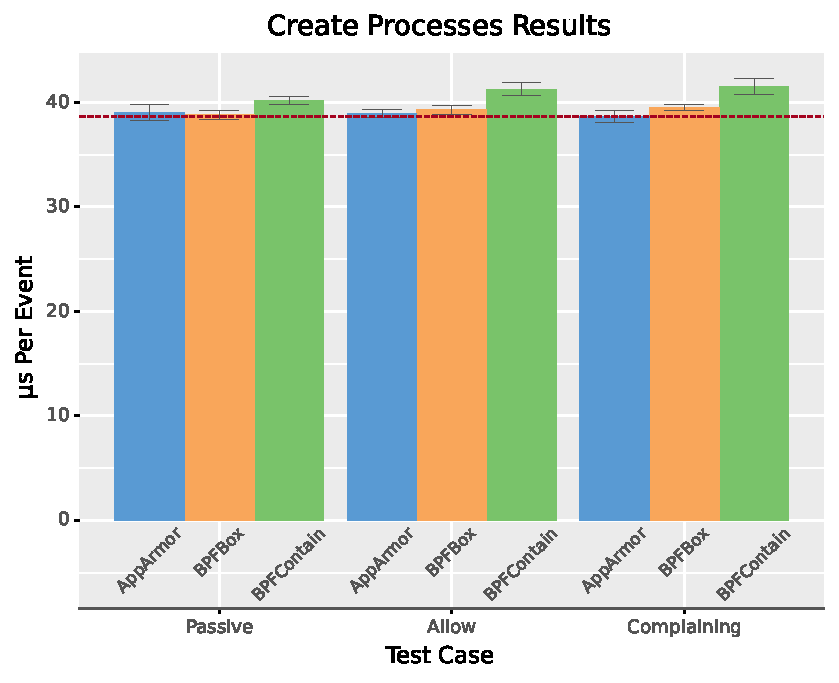
\includegraphics[width=0.45\linewidth]{results/graphs/Create-Processes.pdf}%
  }\\
  \subfloat{
    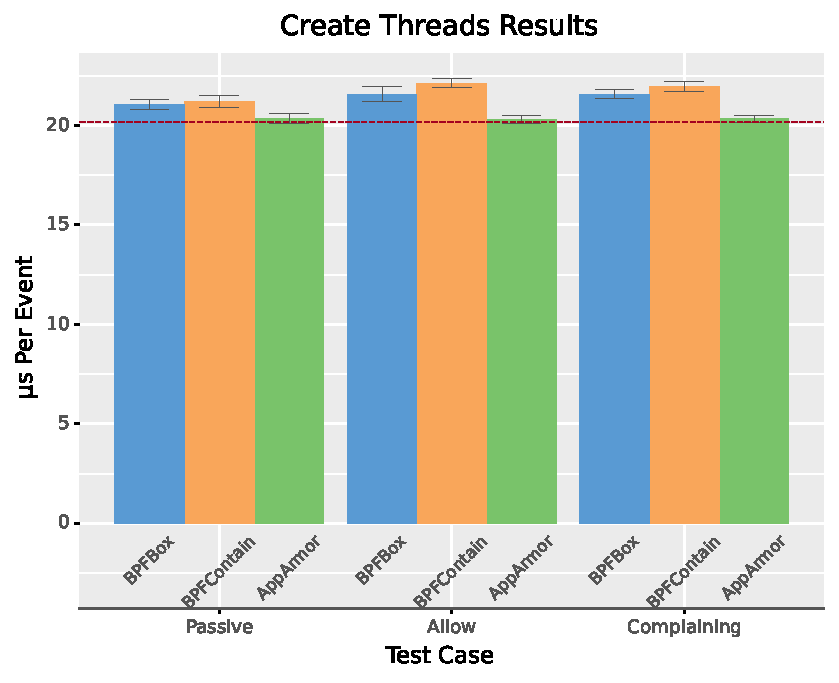
\includegraphics[width=0.45\linewidth]{results/graphs/Create-Threads.pdf}%
  }\qquad
  \subfloat{
    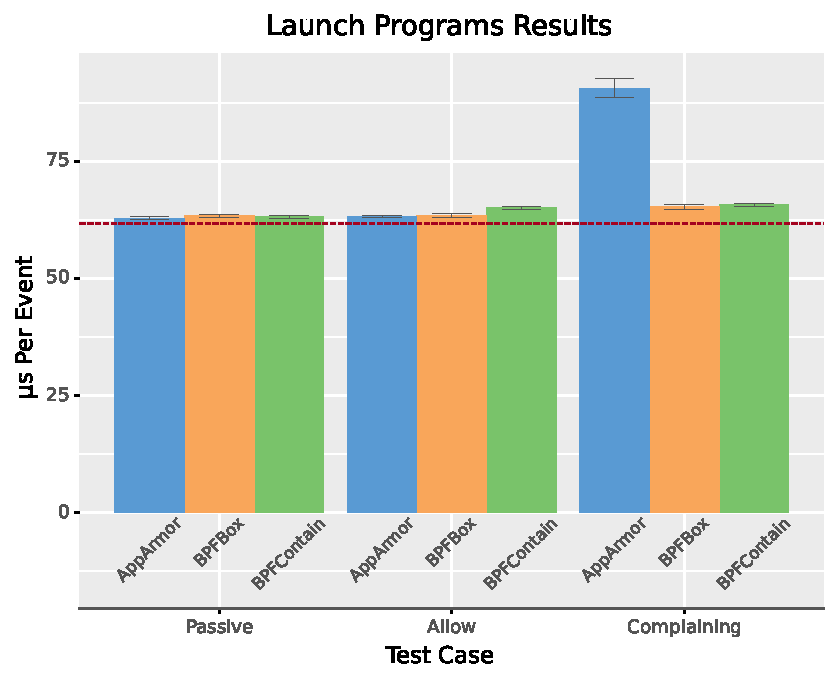
\includegraphics[width=0.45\linewidth]{results/graphs/Launch-Programs.pdf}%
  }\\
  \subfloat{
    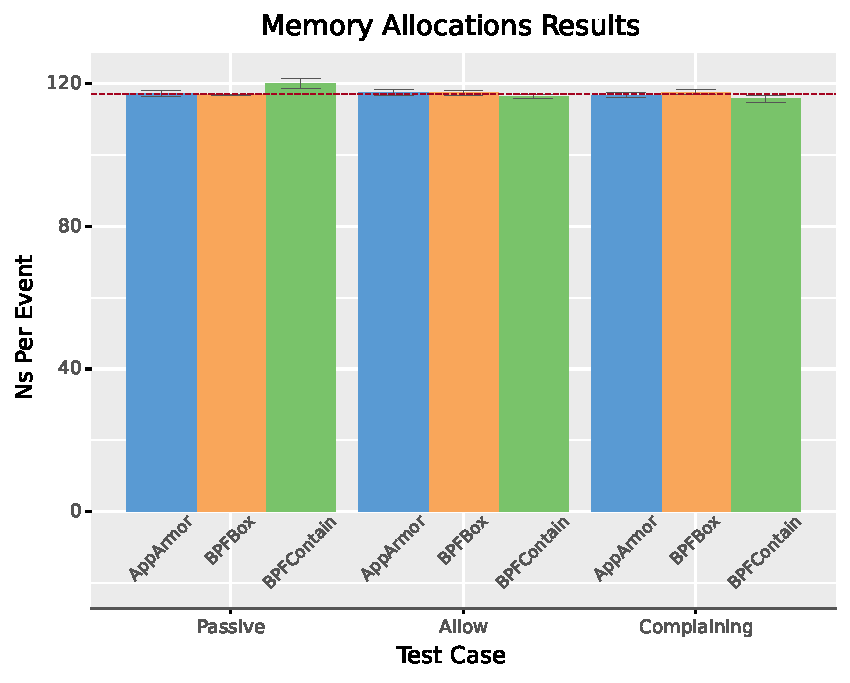
\includegraphics[width=0.45\linewidth]{results/graphs/Memory-Allocations.pdf}%
  }
  \caption{
    The results of the OSBench micro-benchmarks. The error bars show standard
    deviation and the red lines show base measurements for each test. Lower times are
    better.
  }%
  \label{fig:osbench}
\end{figure}

\subsubsection{OSBench File Creation}

The file creation benchmark (\Cref{tab:phoronix-files} and \Cref{fig:osbench}) indicates
that \bpfbox{} and \bpfcontain{} have significantly higher overhead than AppArmor in the
\textbf{Passive} and \textbf{Allow} cases. \bpfcontain{}, in particular, performs the worst
out of the three systems in these two cases. This poor performance can be
explained by the fact that it is an unoptimized research prototype, and that it performs
complex analysis on filesystem operations to come to a policy decision. Conversely,
AppArmor is a well-established security mechanism which has undergone significant
performance optimizations over time. Future optimizations on \bpfcontain{} can
significantly improve its performance overhead in practice. Despite a seemingly high
performance overhead in the \textbf{Passive} and \textbf{Allow} cases, \bpfbox{} and
\bpfcontain{} incur a performance penalty of under 12$\mu$s each, a slowdown which should
be acceptable in practice.  Moreover, in the \textbf{Complain} case, \bpfbox{} and
\bpfcontain{} significantly outperform AppArmor. This result can be attributed to
implementation differences in their event-logging mechanisms.

\begingroup\small
\begin{longtable}[c]{llrrr}
  \caption[Results of the file creation benchmark]{
    Results of the file creation benchmark. Units are $\mu$s per event; lower is
    better. Percent overhead is compared to the baseline result.
  }%
  \label{tab:phoronix-files}\\
  \toprule
   Test Case & System         &  Mean  & Std & Overhead (\%)\\
   \midrule
   Base      & ---            &  42.21 & 1.22 &  ---     \\
   \midrule
   Passive   & \bpfbox{}      &  49.09 & 0.40 &  16.31\% \\
             & \bpfcontain{}  &  48.16 & 0.36 &  14.11\% \\
             & AppArmor       &  43.87 & 0.95 &   3.93\% \\
   \midrule
   Allow     & \bpfbox{}      &  49.41 & 0.39 &  17.08\% \\
             & \bpfcontain{}  &  53.43 & 1.01 &  26.60\% \\
             & AppArmor       &  47.07 & 1.15 &  11.52\% \\
   \midrule
   Complain  & \bpfbox{}      &  50.34 & 0.54 &  19.27\% \\
             & \bpfcontain{}  &  55.67 & 0.75 &  31.89\% \\
             & AppArmor       & 111.66 & 0.75 & 164.55\% \\
  \bottomrule
\end{longtable}
\endgroup

In the \textbf{Passive} case, \bpfbox{} and \bpfcontain{}'s high performance overhead can
be attributed to the fact that they each invoke multiple \gls{bpf} programs over multiple
\gls{lsm} hooks on the \texttt{open(2)}, \texttt{write(2)}, and \texttt{unlink(2)} code
paths. Unlike AppArmor, \bpfbox{} and \bpfcontain{} invoke a new \gls{ebpf} program on
every \gls{lsm} hook along this code path, then perform a map lookup to determine whether
the process is being actively traced. The overhead associated with this many \gls{bpf}
program invocations is non-trivial compared with the overhead of simply calling into an
\gls{lsm} hook. Future improvements to the \gls{krsi} framework may also be able to reduce
the performance overhead of \gls{bpf} \gls{lsm} programs.

In the \textbf{Allow} case, \bpfbox{} is more in line with AppArmor, while \bpfcontain{}
is shown to exhibit a slightly higher overhead. However, as with the \textbf{Passive}
case, this overhead should be acceptable in practice. We can attribute the additional
overhead shown by \bpfcontain{} to the nuances associated with its code path for file and
filesystem policies. For each file operation, \bpfcontain{} performs multiple map queries
and reads information from multiple kernel data structures to enforce its default policy.
Future iterations of \bpfcontain{} may improve this overhead by caching policy decisions
for filesystem objects and/or resolving inefficiencies in how \bpfcontain{} reads
information from kernel data structures.

In the \textbf{Complaining} case, \bpfbox{} and \bpfcontain{} significantly outperform
AppArmor, a fact which can be attributed to inefficiencies in AppArmor's logging
mechanism, which relies on the kernel's audit framework. The ring buffer maps used by
\bpfbox{} and \bpfcontain{} are known to exhibit comparatively less
overhead~\cite{zeng2015_auditing, zhang2021_lsm_file_overhead, nakryiko2020_ringbuf}.
Additional overhead may also arise due to differences in how AppArmor translates files and
access patterns to log messages.

\subsubsection{OSBench Process Creation}

The results of the process creation benchmark (\Cref{tab:phoronix-processes}) indicate
that \bpfbox{} and \bpfcontain{} introduce modest overhead on top of the \texttt{fork(2)}
system call.  Comparatively, AppArmor introduces very little overhead, well within the
margin of error for measurements. The additional overhead introduced by \bpfbox{} and
\bpfcontain{} can be explained by the additional per-process and per-thread accounting
performed by each system. \bpfcontain{}, in particular, handles a significant amount of
per-process and per-thread metadata, which must be populated each time a \texttt{fork(2)}
or \texttt{clone(2)} occurs, and cleaned up each time a process exits. However, it should
be noted that both \bpfbox{} and \bpfcontain{} introduce less than $10\%$ overhead along
this code path (within 1--2$\mu$s), which should be imperceptible in practice.

% \begin{figure}[htp]
%   \centering
%   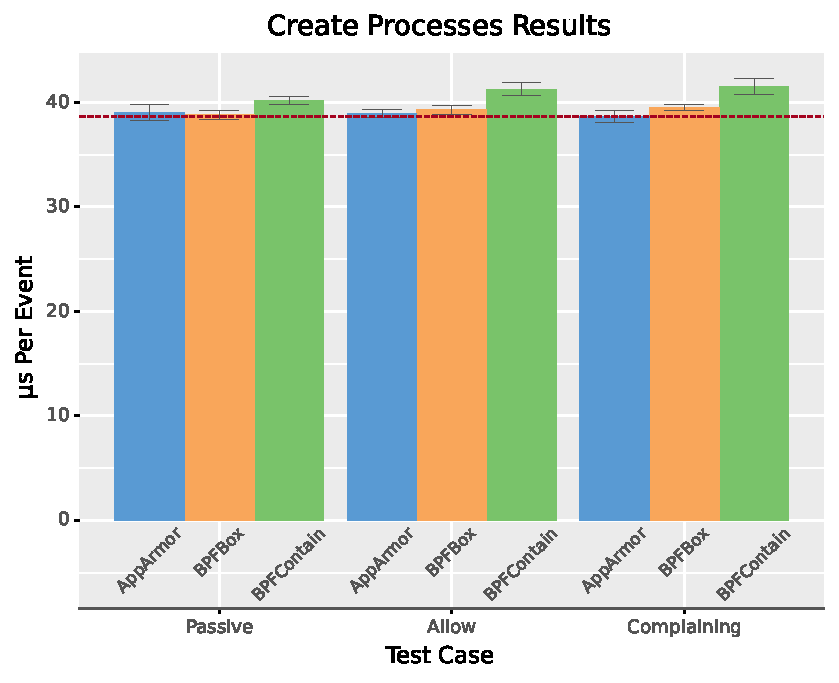
\includegraphics[width=0.8\linewidth]{results/graphs/Create-Processes.pdf}
%   \caption{
%     Results of the process creation benchmark.
%     The error bars show standard deviation and the red line shows the base measurement.
%     Lower times are better.
%   }%
%   \label{fig:phoronix-processes}
% \end{figure}

\begingroup\small
\begin{longtable}[c]{llrrr}
  \caption[Results of the process creation benchmark]{
    Results of the process creation benchmark. Units are $\mu$s per event; lower is
    better. Percent overhead is compared to the baseline result.
  }%
  \label{tab:phoronix-processes}\\
  \toprule
   Test Case & System         &  Mean & Std & Overhead (\%)\\
   \midrule
   Base      & ---            & 38.65 & 0.36 &  ---    \\
   \midrule
   Passive   & \bpfbox{}      & 38.81 & 0.44 &  0.40\% \\
             & \bpfcontain{}  & 40.17 & 0.39 &  3.93\% \\
             & AppArmor       & 39.04 & 0.74 &  1.01\% \\
   \midrule
   Allow     & \bpfbox{}      & 39.28 & 0.41 &  1.63\% \\
             & \bpfcontain{}  & 41.27 & 0.63 &  6.77\% \\
             & AppArmor       & 38.94 & 0.34 &  0.74\% \\
   \midrule
   Complain  & \bpfbox{}      & 39.51 & 0.33 &  2.22\% \\
             & \bpfcontain{}  & 41.49 & 0.76 &  7.33\% \\
             & AppArmor       & 38.68 & 0.56 &  0.07\% \\
  \bottomrule
\end{longtable}
\endgroup

\subsubsection{OSBench Thread Creation}

The thread creation results (\Cref{tab:phoronix-threads}) are directly related to the
process creation results discussed above, insofar as both operations exercise the same
\gls{bpf} programs in \bpfbox{} and \bpfcontain{}. Since thread creation is faster then
process creation, the percentage overhead of \bpfbox{} and \bpfcontain{} appear
comparatively higher, but the underlying delta is the same, at roughly 1--2$\mu$s per
event. Despite these differences in thread and process creation speeds, the resulting
percentage overhead of \bpfbox{} and \bpfcontain{} is still under 10\%.

% \begin{figure}[htp]
%   \centering
%   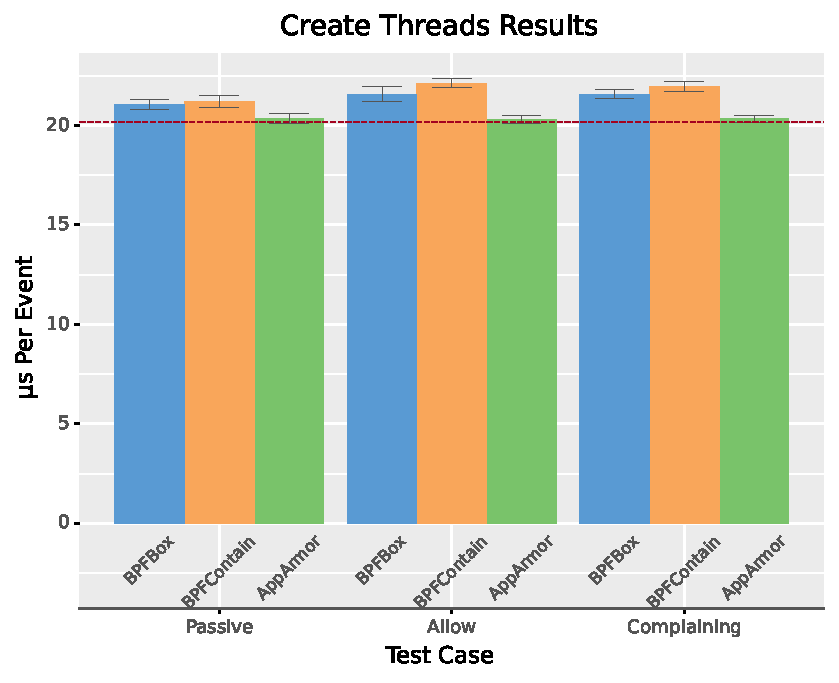
\includegraphics[width=0.8\linewidth]{results/graphs/Create-Threads.pdf}
%   \caption{
%     Results of the thread creation benchmark.
%     The error bars show standard deviation and the red line shows the base measurement.
%     Lower times are better.
%   }%
%   \label{fig:phoronix-threadsa}
% \end{figure}

\begingroup\small
\begin{longtable}[c]{llrrr}
  \caption[Results of the thread creation benchmark]{
    Results of the thread creation benchmark. Units are $\mu$s per event; lower is
    better. Percent overhead is compared to the baseline result.
  }%
  \label{tab:phoronix-threads}\\
  \toprule
   Test Case & System         &  Mean & Std  & Overhead (\%)\\
   \midrule
   Base      & ---            & 20.18 & 0.19 & ---     \\
   \midrule
   Passive   & \bpfbox{}      & 21.06 & 0.25 & 4.37\% \\
             & \bpfcontain{}  & 21.21 & 0.30 & 5.08\% \\
             & AppArmor       & 20.32 & 0.25 & 0.71\% \\
   \midrule
   Allow     & \bpfbox{}      & 21.56 & 0.37 & 6.84\% \\
             & \bpfcontain{}  & 22.11 & 0.22 & 9.53\% \\
             & AppArmor       & 20.29 & 0.18 & 0.54\% \\
   \midrule
   Complain  & \bpfbox{}      & 21.57 & 0.25 & 6.90\% \\
             & \bpfcontain{}  & 21.96 & 0.24 & 8.80\% \\
             & AppArmor       & 20.32 & 0.16 & 0.70\% \\
  \bottomrule
\end{longtable}
\endgroup

\subsubsection{OSBench Program Launching}

The launch programs benchmark (\Cref{tab:phoronix-launch-programs}) is essentially the
same as the process creation benchmark (c.f.~\Cref{tab:phoronix-processes}), with one
major difference: the addition of an \texttt{execve(2)} call after the \texttt{clone(2)}
system call. This \texttt{execve(2)} call adds a constant overhead of about 20$\mu$s on
top of the original process creation results, as well as additional \gls{lsm} hook
invocations along the \texttt{execve(2)} code path. These factors contribute to \bpfbox{}
and \bpfcontain{} performing slightly worse than AppArmor in the \textbf{Passive} and
\textbf{Allow} cases and significantly better than AppArmor in the \textbf{Complaining}
case.

The additional \gls{lsm} hook invocations caused by the \texttt{execve(2)} severely impact
AppArmor's performance in the \textbf{Complaining} case, for the same reasons as discussed
in the file creation results (c.f.~\Cref{tab:phoronix-files}). \bpfbox{} and \bpfcontain{}
exhibit comparatively little overhead, despite the \texttt{execve(2)} call. This result
can be explained by the fact that \texttt{execve(2)}'s code path invokes significantly
fewer \gls{lsm} hooks than the file creation and deletion code paths we examined earlier.
In all test cases, \bpfbox{} and \bpfcontain{} are able to achieve under $7\%$ overhead in
the worst case, and under $3\%$ in the majority of cases.

% \begin{figure}[htp]
%   \centering
%   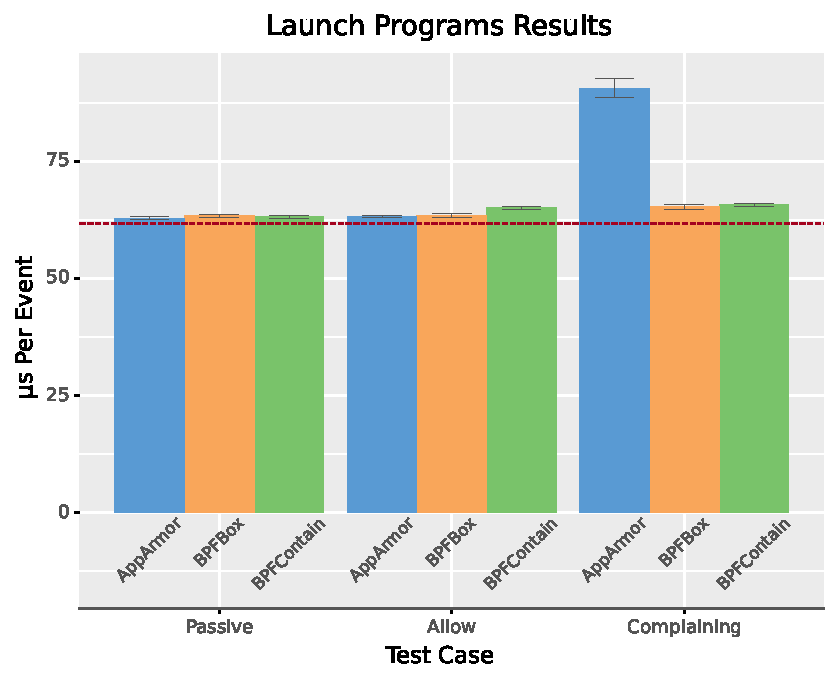
\includegraphics[width=0.8\linewidth]{results/graphs/Launch-Programs.pdf}
%   \caption{
%     Results of the program launching benchmark.
%     The error bars show standard deviation and the red line shows the base measurement.
%     Lower times are better.
%   }%
%   \label{fig:phoronix-launch-programs}
% \end{figure}

\begingroup\small
\begin{longtable}[c]{llrrr}
  \caption[Results of the program launching benchmark]{
    Results of the program launching benchmark. Units are $\mu$s per event; lower is
    better. Percent overhead is compared to the baseline result.
  }%
  \label{tab:phoronix-launch-programs}\\
  \toprule
   Test Case & System         &  Mean & Std  & Overhead (\%)\\
   \midrule
   Base      & ---            & 61.67 & 0.20 & ---     \\
   \midrule
   Passive   & \bpfbox{}      & 63.30 & 0.28 & 2.64 \% \\
             & \bpfcontain{}  & 63.12 & 0.28 & 2.34 \% \\
             & AppArmor       & 62.84 & 0.25 & 1.89 \% \\
   \midrule
   Allow     & \bpfbox{}      & 63.44 & 0.40 & 2.86 \% \\
             & \bpfcontain{}  & 65.05 & 0.38 & 5.47 \% \\
             & AppArmor       & 63.17 & 0.21 & 2.43 \% \\
   \midrule
   Complain  & \bpfbox{}      & 65.22 & 0.48 & 5.75 \% \\
             & \bpfcontain{}  & 65.66 & 0.30 & 6.47 \% \\
             & AppArmor       & 90.56 & 1.97 & 46.83\% \\
  \bottomrule
\end{longtable}
\endgroup

\subsubsection{OSBench Memory Allocations}

The memory allocation benchmark (\Cref{tab:phoronix-memory}) indicates that none of the
systems had any significant affect on memory allocation. In some cases, percent overhead
falsely appears to indicate a performance \textit{improvement}, which we attribute to
measurement error rather than any indication of increased performance. This result is
consistent with expectations, since memory allocation does not directly interact with any
\gls{lsm} hooks in the kernel, and neither \bpfbox{} nor \bpfcontain{} instruments any
\gls{bpf} programs on the heap allocation code path.

% \begin{figure}[htp]
%   \centering
%   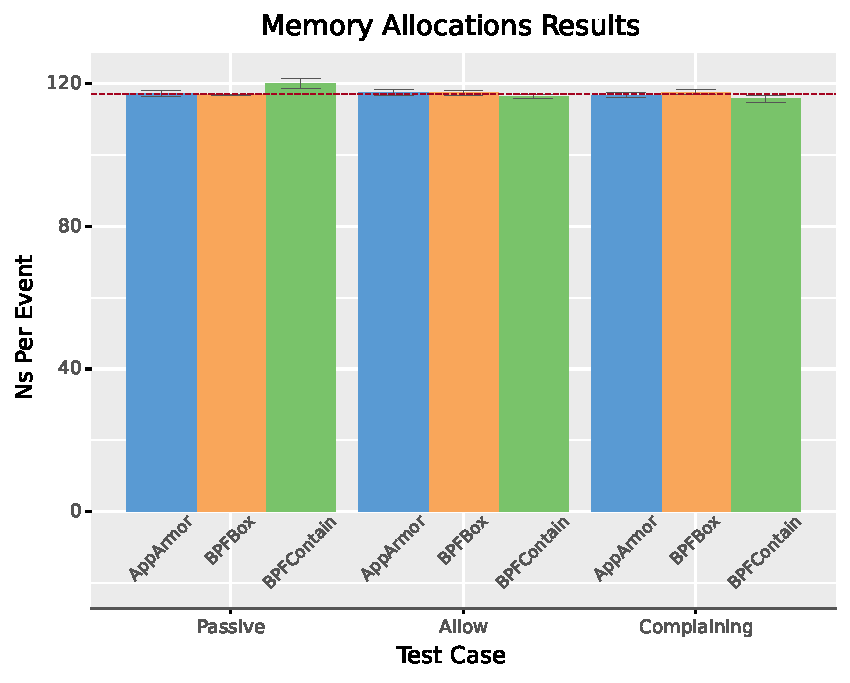
\includegraphics[width=0.8\linewidth]{results/graphs/Memory-Allocations.pdf}
%   \caption{
%     Results of the memory allocation benchmark.
%     The error bars show standard deviation and the red line shows the base measurement.
%     Lower times are better.
%   }%
%   \label{fig:phoronix-memory}
% \end{figure}

\begingroup\small
\begin{longtable}[c]{llrrr}
  \caption[Results of the memory allocation benchmark]{
    Results of the memory allocation benchmark. Units are Ns per event; lower is
    better. Percent overhead is compared to the baseline result.
  }%
  \label{tab:phoronix-memory}\\
  \toprule
   Test Case & System         &  Mean  & Std  & Overhead (\%)\\
   \midrule
   Base      & ---            & 117.17 & 0.67 & ---     \\
   \midrule
   Passive   & \bpfbox{}      & 116.87 & 0.18 & -0.26\% \\
             & \bpfcontain{}  & 120.05 & 1.27 &  2.46\% \\
             & AppArmor       & 117.24 & 0.97 &  0.06\% \\
   \midrule
   Allow     & \bpfbox{}      & 117.41 & 0.71 &  0.21\% \\
             & \bpfcontain{}  & 116.42 & 0.62 & -0.64\% \\
             & AppArmor       & 117.49 & 0.81 &  0.28\% \\
   \midrule
   Complain  & \bpfbox{}      & 117.62 & 0.75 &  0.38\% \\
             & \bpfcontain{}  & 115.73 & 1.04 & -1.22\% \\
             & AppArmor       & 116.81 & 0.80 & -0.31\% \\
  \bottomrule
\end{longtable}
\endgroup


\subsubsection{Kernel Compilation Results}

The kernel compilation benchmark (\Cref{tab:phoronix-kernel}) provides a representative
depiction of overhead for a computationally-heavy task that involves multiple processes
and significant amounts of file I/O. The results of this benchmark indicate that \bpfbox{}
and \bpfcontain{} exhibit performance overhead that is roughly consistent with AppArmor in
the average case. The \textbf{Passive} and \textbf{Allow} results indicate that all three
systems exhibit an acceptable performance overhead of under about $3\%$. The
\textbf{Complain} results indicate that \bpfcontain{} performs significantly better than
both \bpfbox{} and AppArmor under a large event logging volume. This result can be
attributed to minor implementation details, including improvements in how \bpfcontain{}
handles event logging from multiple distinct sources.
%This result can likely be
%attributed to \bpfcontain{}'s more efficient userspace implementation in Rust, which
%significantly outperforms the \bpfbox{} Python implementation.

\begingroup\small
\begin{longtable}[c]{llrrr}
  \caption[Results of the kernel compilation benchmark]{
    Results of the kernel compilation benchmark. Units are seconds to compile; lower is
    better. Percent overhead is compared to the baseline result.
  }%
  \label{tab:phoronix-kernel}\\
  \toprule
   Test Case & System         &  Mean  & Std  & Overhead (\%)\\
   \midrule
   Base      & ---            & 235.32 & 1.96 & ---     \\
   \midrule
   Passive   & \bpfbox{}      & 237.95 & 1.88 &  1.12\% \\
             & \bpfcontain{}  & 237.63 & 2.08 &  0.98\% \\
             & AppArmor       & 236.45 & 1.92 &  0.48\% \\
   \midrule
   Allow     & \bpfbox{}      & 238.23 & 2.19 &  1.24\% \\
             & \bpfcontain{}  & 243.09 & 2.19 &  3.30\% \\
             & AppArmor       & 237.59 & 2.04 &  0.97\% \\
   \midrule
   Complain  & \bpfbox{}      & 269.64 & 1.98 & 14.59\% \\
             & \bpfcontain{}  & 244.81 & 2.04 &  4.03\% \\
             & AppArmor       & 288.54 & 2.11 & 22.62\% \\
  \bottomrule
\end{longtable}
\endgroup

\begin{figure}[p]
  \centering
  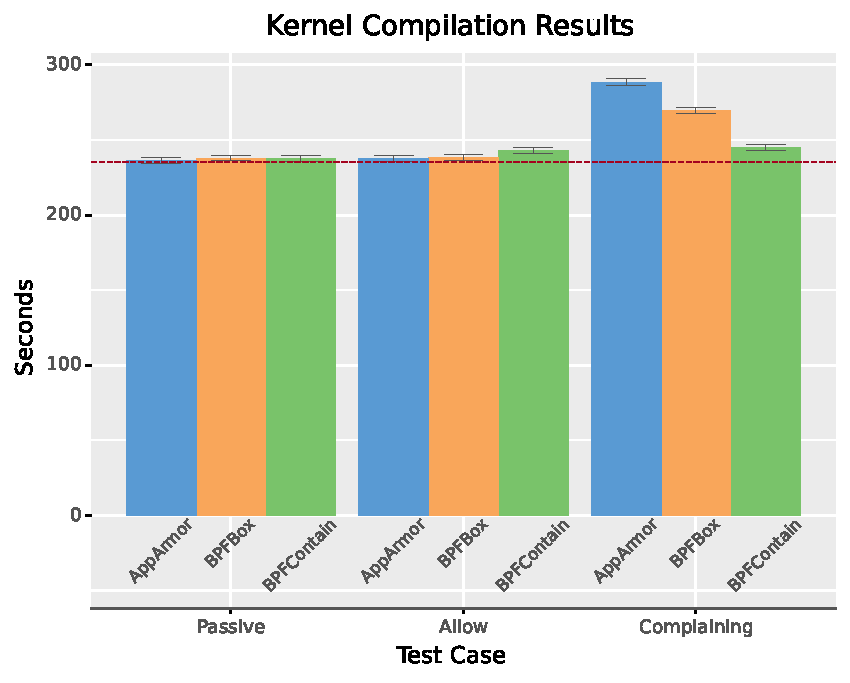
\includegraphics[width=0.6\linewidth]{results/graphs/Kernel-Compilation.pdf}
  \caption{
    Results of the kernel compilation benchmark.
    The error bars show standard deviation and the red line shows the base measurement.
    Lower times are better.
  }%
  \label{fig:phoronix-kernel}
\end{figure}

\begin{figure}[p]
  \centering
  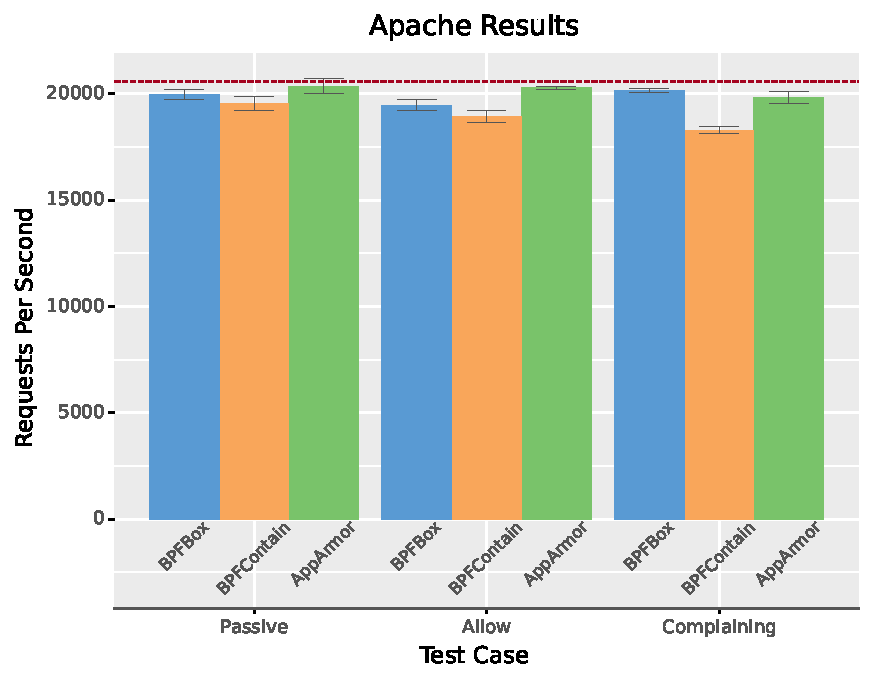
\includegraphics[width=0.6\linewidth]{results/graphs/Apache.pdf}
  \caption{
    Results of the Apache web server benchmark.
    The error bars show standard deviation and the red line shows the base measurement.
    Higher requests per second are better.
  }%
  \label{fig:phoronix-apache}
\end{figure}


\subsubsection{Apache Web Server Results}

The Apache web server benchmark (\Cref{tab:phoronix-apache}) indicates that, while
\bpfbox{} and \bpfcontain{} do exhibit a higher performance overhead than AppArmor, this
overhead is still within an acceptable range at around $11\%$ in the worst case for
\bpfcontain{}. This overhead should still be quite acceptable in practice, and can be
improved through further optimizations in \bpfcontain{}'s enforcement engine, which is
still in the prototype phase. The results from the \textbf{Complain} case appear to
indicate a slight performance improvement for \bpfbox{} over AppArmor; this is likely due
to variance in the measurements rather than a true performance improvement, as the
difference between the two systems falls within the margin of error.

\begingroup\small
\begin{longtable}[c]{llrrr}
  \caption[Results of the Apache web server benchmark]{
    Results of the Apache web server benchmark. Units are requests per second; higher is
    better. Percent overhead is compared to the baseline result.
  }%
  \label{tab:phoronix-apache}\\
  \toprule
   Test Case & System         &  Mean   & Std   & Overhead (\%)\\
   \midrule
   Base      & ---            & 20576.49 & 281.94 & ---     \\
   \midrule
   Passive   & \bpfbox{}      & 19946.04 & 233.62 &  3.06\% \\
             & \bpfcontain{}  & 19530.92 & 317.95 &  5.08\% \\
             & AppArmor       & 20363.42 & 331.64 &  1.04\% \\
   \midrule
   Allow     & \bpfbox{}      & 19465.86 & 253.81 &  5.40\% \\
             & \bpfcontain{}  & 18934.55 & 299.23 &  7.98\% \\
             & AppArmor       & 20276.95 &  64.30 &  1.46\% \\
   \midrule
   Complain  & \bpfbox{}      & 20139.10 & 101.59 &  2.13\% \\
             & \bpfcontain{}  & 18293.09 & 160.00 & 11.10\% \\
             & AppArmor       & 19827.05 & 298.27 &  3.64\% \\
  \bottomrule
\end{longtable}
\endgroup

% \subsubsection{\glsentryshort{ipc} Results}

\subsection{Discussion of Results}%
\label{ss:eval-performance-discussion}

The results of the benchmarking tests show that both \bpfbox{} and \bpfcontain{} incur
acceptable performance overhead in practice. In many cases, overhead is competitive with
AppArmor, a standard \gls{lsm} that ships with the stock Linux kernel. In other cases, the
performance overhead of \bpfbox{} and \bpfcontain{} is higher than that of AppArmor, but
still within an acceptable range, such that the slowdown should be either imperceptible or
acceptable in most practical use cases.  As \bpfbox{} and \bpfcontain{} are both research
prototypes, they have not yet been optimized to the extent that AppArmor has. This lack of
optimization is particularly evident in the results for \bpfcontain{}, and may account for
significant differences in performance in the file I/O and Apache web server tests.

While \bpfbox{} and \bpfcontain{} are not as efficient as AppArmor in the \textbf{Passive}
and \textbf{Allow}  test cases, the additional performance overhead should be an
acceptable price to pay for the increase in flexibility and system observability afforded
by an \gls{ebpf} implementation as opposed to a traditional Linux Security Module.
Moreover, \bpfcontain{} extends \bpfbox{}'s original enforcement model, adding new rule categories
and enforcement defaults. While these enhancements may be the cause of some additional
performance overhead, we attribute the majority of \bpfcontain{}'s actual performance
overhead to sub-optimal memory allocations and data structure access patterns, which can
be optimized in the future.

Despite under-performing in the \textbf{Passive} and \textbf{Allow} cases, both \bpfbox{}
and \bpfcontain{} significantly outperform AppArmor in the \textbf{Complain} test case,
due to a more efficient event logging mechanism.  \Cref{tab:phoronix-geometric} shows the
geometric mean of all tests for each test case, indicating that \bpfbox{} and
\bpfcontain{} exhibit and average performance penalty of under $9\%$ in practice, while
AppArmor can exhibit overheads of up to $20\%$ in the worst case.

\begin{table}[htp]
  \centering
  \caption[Geometric means of Phoronix benchmarking results]{
    Geometric means of Phoronix benchmarking results. These are indicative of over all
    performance across all tests. For test case, percent change from the base results are
    also given. Higher values are better.
  }%
  \label{tab:phoronix-geometric}
  \begin{tabular}{llrr}
  \toprule
   Test Case & System        & Geom. Mean & Overhead (\%)\\
   \midrule
   Base      &               & 6.238          & --- \\
   \midrule
   Passive   & \bpfbox{}     & 6.007          & 3.70\% \\
             & \bpfcontain{} & 5.951          & 4.60\% \\
             & AppArmor      & 6.158          & 1.28\% \\
   \midrule
   Allow     & \bpfbox{}     & 5.944          & 4.71\% \\
             & \bpfcontain{} & 5.763          & 7.61\% \\
             & AppArmor      & 6.086          & 2.35\% \\
   \midrule
   Complain  & \bpfbox{}     & 5.823          & 6.65\% \\
             & \bpfcontain{} & 5.693          & 8.74\% \\
             & AppArmor      & 4.962          & 20.46\% \\
  \bottomrule
  \end{tabular}
\end{table}

Although the results presented in this section indicate a comparative performance with
AppArmor, many other widely-adopted \glspl{lsm} can perform significantly worse than
AppArmor in some cases. For instance, Zhang \etal~\cite{zhang2021_lsm_file_overhead} found
that SELinux, perhaps the most widely-used Linux \gls{mac} implementation, exhibits
significant performance overhead, many times worse than AppArmor in some cases. These
results could indicate that \bpfbox{} and \bpfcontain{} might perform favourably compared
to alternative \glspl{lsm} like SELinux, although further investigation is needed in order
to establish a direct comparison.

\section{Security Analysis}%
\label{s:eval-security}

We now turn our attention to the security of \bpfbox{} and \bpfcontain. Specifically, we
conduct an informal security analysis on both systems, evaluating how well they are able
to confine an attacker under the threat model presented in \Cref{s:cp-threat-model} of
\Cref{c:confinement-problem}. In particular, we examine the various policy rule categories
provided by both \bpfbox{} and \bpfcontain{} as well as how their respective enforcement
engines enforce policy at runtime. We characterize an adversary's ability to escape
confinement based on whether the adversary is able to violate the security assumptions of
\bpfbox{} and \bpfcontain{} under a policy designed to prevent such violations.

% \todo{The plan for this section is to first revisit the threat model, then go through each
% policy \enquote{category} supported by \bpfbox{} and \bpfcontain{}. In a few categories
% (IPC, capabilities, kernel interfaces) \bpfcontain{} is just better... The \bpfbox{}
% prototype left some of this stuff out, and some of it is much weaker. In the networking
% category, both \bpfbox{} and \bpfcontain{} have room for improvement. We can do a forward
% ref to limitations / future work for this.}

\subsection{Threat Model Revisited}

Recall the threat model presented in \Cref{s:cp-threat-model} of
\Cref{c:confinement-problem}. We assume a remote adversary who is confined by some policy
$\mathcal{P}$. The adversary's goal is to escape confinement by circumventing
$\mathcal{P}$, enabling them to access sensitive resources, interfere or tamper with the
system, or perform other unauthorized actions. Our goal is to confine the adversary,
limiting the set of all actions they can perform to some subset of allowed actions. We
express such confinement using the policy $\mathcal{P}$ which defines rules governing the
set of operations some subject $\mathcal{S}_i$ may perform on system objects
$\mathcal{O}_1 \mathellipsis \mathcal{O}_n$. To enforce our confinement policy, we rely on
a \textit{confinement engine} which has been loaded into the kernel's reference monitor.

Under our threat model, we assign significant capabilities to the adversary. Aside from the
restrictions imposed by our confinement policy, we assume that they have root-level access
to the system, including the ability to load code into the kernel, bypass discretionary
access controls, read or modify any persistent resource, and establish persistent access
to the system. Thus, an attacker that is able to escape or bypass confinement has
effectively compromised the entire system. Further, our enforcement engine must take steps
protect itself, preventing the attacker from simply loading or modifying code in the
kernel, which would result in the ability to tamper with or bypass the enforcement engine.

In the subsections that follow, we consider four broad access categories and describe how
\bpfbox{} and \bpfcontain{}'s confinement policy and enforcement engine prevent attacks
related to these access categories. In some cases, the original \bpfbox{} policy
specification (as presented in this thesis) provided insufficient protection against
specific access patterns. In these instances, we describe how \bpfcontain{} improves upon
the original \bpfbox{} design.

\subsection{Files and Filesystems}

Correct mediation of file and filesystem accesses is critical to ensure that an adversary
is confined. Files define the canonical persistent data store in modern \gls{cots}
operating systems, including Linux. Depending on the nature of the file, the information
stored within may be confidential, security-sensitive, or otherwise critical to normal
system operation. Attacker modification of persistent files is often the first step in
mounting a Confused Deputy attack~\cite{hardy1988_confused_deputy}, along with other
classes of attack such as \gls{toctou} race conditions, data corruption, and memory safety
attacks.

Under the Unix model, special files and filesystems define an entrypoint into kernel
interfaces, many of which are security-sensitive. For example, character devices expose an
interface into device drivers, while special filesystems like \texttt{sysfs} and
\texttt{securityfs} expose behavioural parameters and export sensitive information such as
the system memory map. Limiting access to these files is of paramount importance, since
unrestricted access could enable an attacker to change the behaviour of the kernel, read
sensitive information, or modify global system parameters.

\subsubsection{\bpfbox{}}

To confine a process' access to the filesystem, \bpfbox{} supports \enquote{file} rules,
which take a pathname and corresponding access vector. This access vector encodes the
specific file operations that a process can perform on the file. Since \bpfbox{} policies
are default-deny, an adversary running under a \bpfbox{} confinement policy should be
unable to perform an operation $Op_i$ on any file $F_j$ unless this operation is
explicitly covered under a file rule. For the purposes of confinement, \bpfbox{} treats
all files equally, regardless of whether the file is a special file or belongs to
a special filesystem. Thus, any access to any file on the system is governed by the same
set of file rules. The only exception to this is a special \enquote{proc} rule which
enables a policy to define access to per-pid \texttt{procfs} entries belonging to another
process.

To enforce its file policy, the \bpfbox{} enforcement engine instruments \gls{ebpf}
programs on several \gls{lsm} hooks, including inode-based, file-based, and path-based
hooks. Taken together, these hooks provide complete mediation over the set of all file
operations, by instrumenting access at the \gls{vfs} layer. \bpfbox{} encodes its file
policy using an \gls{ebpf} map, taking the inode and device numbers associated with a file
and its filesystem as a key. When a process requests access to a file, \bpfbox{} computes
a key for that file and makes a query against its policy map. Although this is an
effective method of uniquely identifying a file, its security is subject to a few inherent
limitations. An attack against this model would consist of unlinking and re-creating a file after
a policy has been loaded, causing \bpfbox{} to see it as a different file when enforcing
access control. In the worst case, this is effectively a denial of service against the
confined process, since \bpfbox{} enforces a default-deny policy on unrecognized files.
This attack would also require the adversary to be unconfined, such that they would be
able to perform the necessary operations on the file.

\subsubsection{\bpfcontain{}}

Like \bpfbox{}, \bpfcontain{} supports file rules that specify a target pathname and
corresponding access vector. In addition to file rules, \bpfcontain{} also supports
filesystem rules for defining per-filesystem policy. A filesystem rule can be thought of
as a coarser-grained version of a file rule, specifying access at the per-filesystem
rather than the per-file level. In order to ensure mediation over explicit denials,
\bpfcontain{} always prioritizes fine-grained file rules over coarse-grained filesystem
rules.  This prevents a policy from inadvertently obviating its own file rules with
a careless filesystem rule.

Unlike \bpfbox{}, \bpfcontain{} treats regular files differently from special files and
special filesystems.

\subsection{Capabilities}

\subsubsection{\bpfbox{}}

\subsubsection{\bpfcontain{}}

\subsection{Networking}

\subsubsection{\bpfbox{}}

\subsubsection{\bpfcontain{}}

\subsection{\glsentryshort{ipc}}

\subsubsection{\bpfbox{}}

\subsubsection{\bpfcontain{}}



\section{Summary}%
\label{s:eval-summary}
